\documentclass[../midgard.tex]{subfiles}
\graphicspath{{\subfix{../images/}}}
\begin{document}

\section{Time model}
\label{h:time-model}

Midgard partitions time in two different ways:
\begin{description}
    \item[Operator shifts.] Predefined, non-overlapping time intervals assigned to operators by the Midgard scheduler.
      Each operator has the exclusive privilege to commit blocks to the state queue and resolve nodes in the settlement queue during their assigned shifts.
      If an operator fails to commit blocks regularly in their shift, the next operator can take over.
    \item[Event intervals.] Emergent, non-overlapping time intervals claimed by operators' committed blocks.
      Each operator block is expected to include all user events with inclusion times within its event interval and to exclude all other user events.
      For L1 user events (deposits, transaction orders, withdrawal orders), this is enforced by Midgard's ledger rules.
\end{description}

Operator shifts are evenly sized according to the \code{shift\_duration} Midgard protocol parameter.
The scheduler assigns operators to shifts by iterating over the list of active operators in key-descending order, allowing new operators into the list at the end of each cycle.
The state queue enforces this schedule by requiring the time-validity upper bound of every block commitment transaction to fall within its operator's shift.

Each block's event interval is between the previous block's time-validity upper bound and its own time-validity upper bound.
The block's time-validity lower bound is irrelevant to Midgard's consensus protocol because the causal relationship between blocks is determined by the forward links between state queue nodes, as well as the backwards links between block headers.
An operator is free to submit blocks at a rapid cadence during their shift.%
\footnote{Indeed, an operator may commit blocks without waiting for L1 confirmation.
As long as the blocks are valid, no one can interfere with the operator's chain of block commitment transactions.
Moreover, if operators coordinate their activity offchain, this rapid cadence can be mostly maintained across shift boundaries.}

\begin{figure}[htb]
\centering
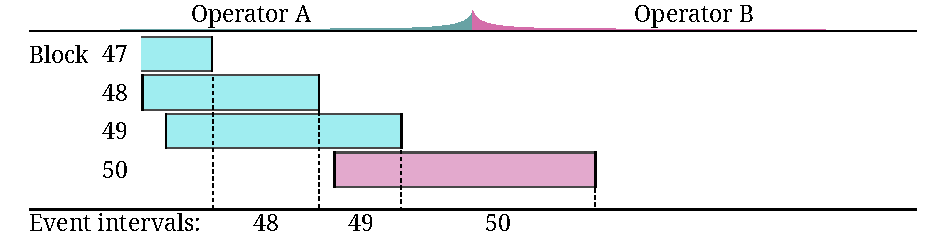
\includegraphics[scale=1]{\subfix{../images/time-model.pdf}}
\caption{Midgard time model.
Each rectangle shows a block's time-validity interval.
  The color indicates the operator who must have committed the block.
  The top axis shows the operator shifts.
  The bottom axis shows the event intervals.
  }
\label{fig:time-model}
\end{figure}

\end{document}
